%% -*- coding: utf-8 -*-
\documentclass[14pt,a4paper]{scrartcl} 
\usepackage[utf8]{inputenc}
\usepackage[english,russian]{babel}
\usepackage{indentfirst}
\usepackage{misccorr}
\usepackage{graphicx}
\usepackage{amsmath}
\usepackage{listings}
\begin{document}
\tableofcontents
\newpage
\section{Введение}
Для разработки алгоритма использовалась среда разработки Visual Studio (в дальнейшем VS) на языке прогроммирования С++. При открытии VS запускается следующее окно (рисунок 1):
\begin{figure}[h!]
    \centering
    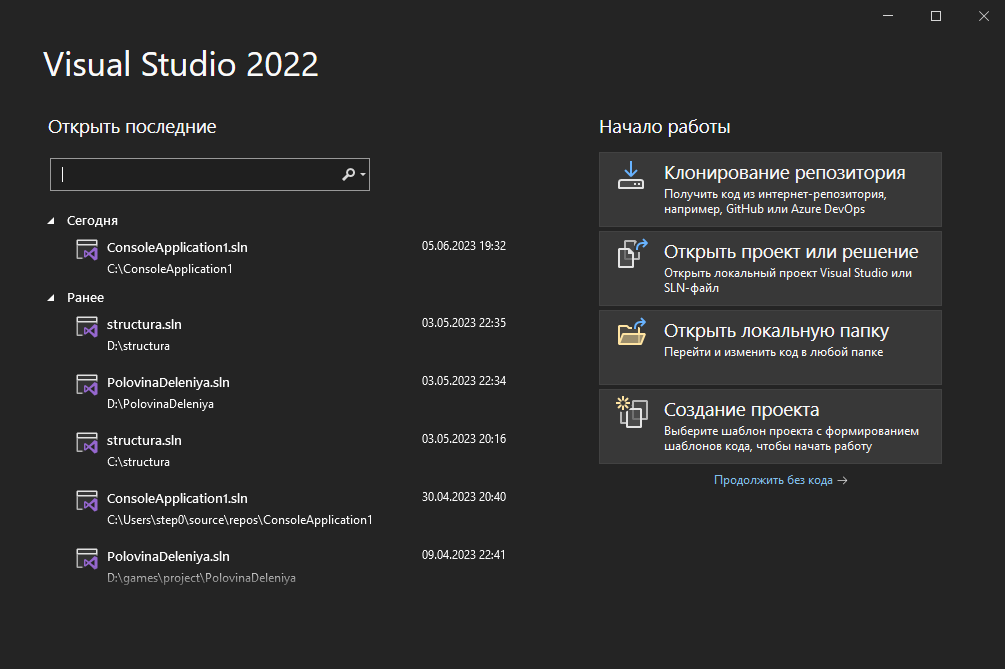
\includegraphics [width=0.9\textwidth]{pic1}\\
    \caption{Окно запуска проектов Visual Studio}
    \label{fig:pic1}
\end{figure}

\newpage

Для отрытия проекта необходимо кликнуть на нужное наименование после чего проект благополучно запуститься и можно начинать редактирование и компиляцию кода (рисунок 2): 

\begin{figure}[h!]
    \centering
    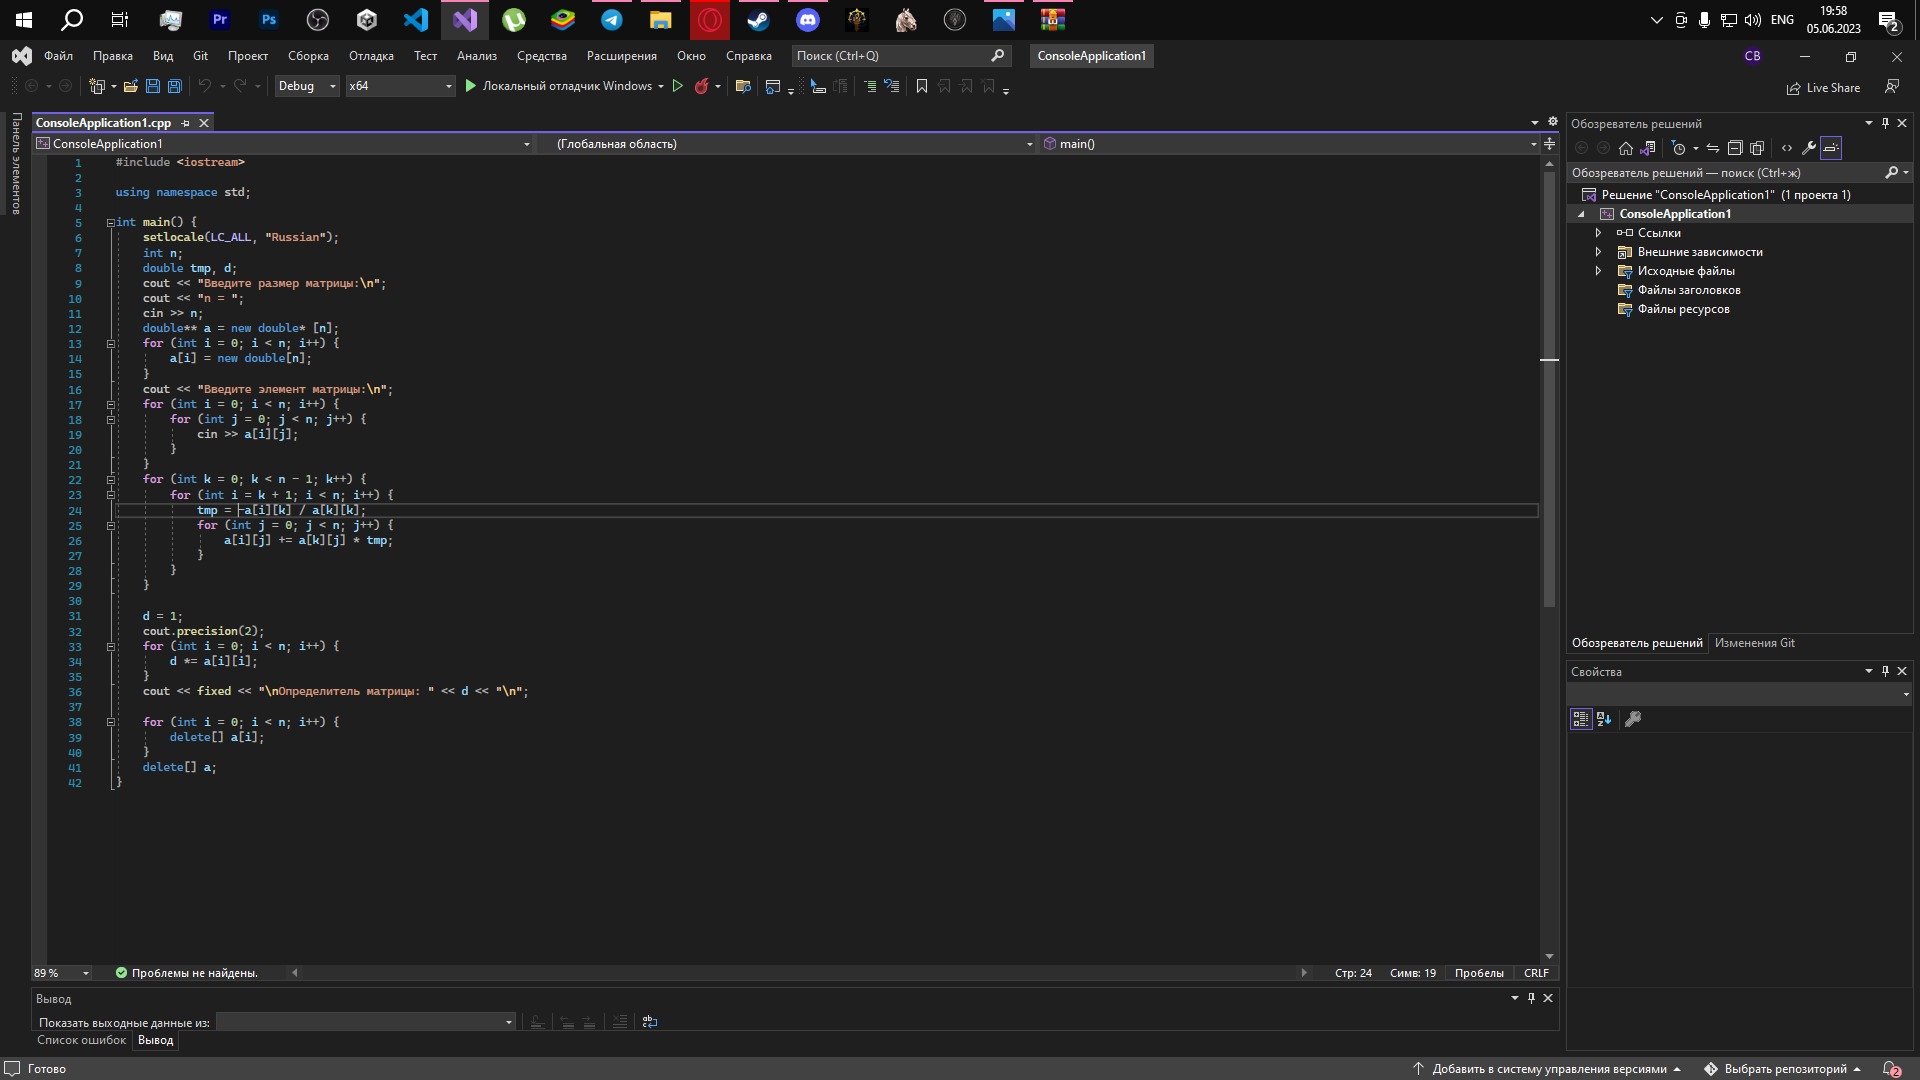
\includegraphics [width=0.9\textwidth]{pic2}\\
    \caption{Окно проекта Visual Studio}
    \label{fig:pic2}
\end{figure}

\newpage
\section{Работа программы}
На рисунке 2 можно увидеть алгоритм решения задачи на нахождение определителя матрицы методом Гаусса. Результат его работы отображён на рисунке 3:

\begin{figure}[h!]
    \centering
    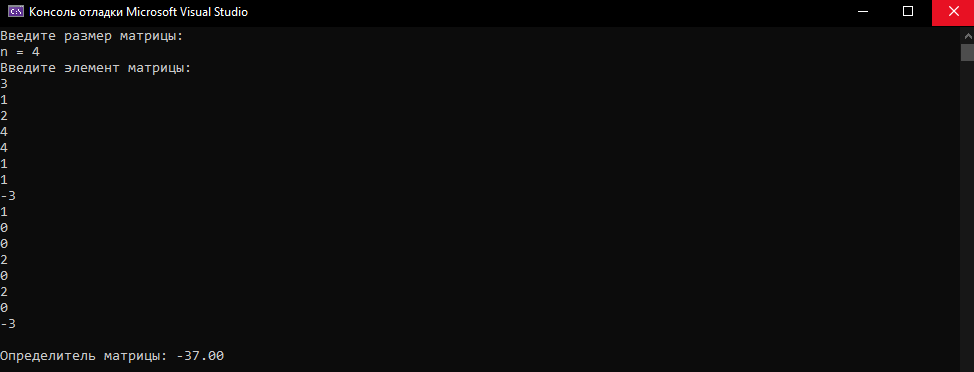
\includegraphics [width=0.9\textwidth]{pic3}\\
    \caption{Окно проекта Visual Studio}
    \label{fig:pic3}
\end{figure}
\section{Код программы}


\begin{lstlisting} 
#include <iostream>

using namespace std;

int main() {
    setlocale(LC_ALL, "Russian");
    int n;
    double tmp, d;
    cout << "Enter the size of the matrix: ";
    cout << "n = ";
    cin >> n;
    double** a = new double* [n];
    for (int i = 0; i < n; i++) {
        a[i] = new double[n];
    }
    cout << "Enter the matrix element: ";
    for (int i = 0; i < n; i++) {
        for (int j = 0; j < n; j++) {
            cin >> a[i][j];
        }
    }
    for (int k = 0; k < n - 1; k++) {
        for (int i = k + 1; i < n; i++) {
            tmp = -a[i][k] / a[k][k];
            for (int j = 0; j < n; j++) {
                a[i][j] += a[k][j] * tmp;
            }
        }
    }
    
    d = 1;
    cout.precision(2);
    for (int i = 0; i < n; i++) {
        d *= a[i][i];
    }
    cout << fixed << "Matrix determinant: " << d << "\n";

    for (int i = 0; i < n; i++) {
        delete[] a[i];
    }
    delete[] a;
}
\end{lstlisting}

\newpage
\section{Список используемой литературы}

\begin{enumerate}

    \item Оосновы алгоритмизации и программирования, Т.А. Жданова, Ю.С. Бузыкова, 2011. - 59 с.
\end{enumerate}

\end{document}
